\documentclass[11pt, a4paper]{article}
\usepackage{graphicx, fullpage, hyperref, listings}
\usepackage{appendix, pdfpages, color}
\usepackage{indentfirst} %段首空两格 棒
\usepackage{chngpage} 
\usepackage{tocloft}            % This squashes the Table of Contents a bit
\usepackage{pdfpages}
\usepackage{multirow}
\usepackage{amsmath}
\usepackage{amssymb}
\usepackage{framed}
%\usepackage{math}
%% Used on windows
%\usepackage[UTF8]{ctex}
%\usepackage{array}%需要该宏包

%% Used On Ubuntu
\usepackage{CJKutf8}


\setlength\cftbeforesecskip{3pt}
\renewcommand{\contentsname}{\centerline{\textbf{Content}}}
\graphicspath{{images/}}

\usepackage{multicol}

\usepackage{graphicx}
\usepackage{epstopdf}
\hypersetup{CJKbookmarks,%
	bookmarksnumbered,%
	colorlinks,%
	linkcolor=black,%
	citecolor=black,%
	plainpages=false,%
	pdfstartview=FitH}

%%%%%%%代码语法高亮设置

\usepackage{color}

\definecolor{pblue}{rgb}{0.13,0.13,1}
\definecolor{pgreen}{rgb}{0,0.5,0}
\definecolor{pred}{rgb}{0.9,0,0}
\definecolor{pgrey}{rgb}{0.46,0.45,0.48}

\usepackage{listings}
\lstset{
	language=Java,
	showspaces=false,
	showtabs=false,
	%%%%%
	frame = single,
	stepnumber = 2,  
	numbersep = 4pt, 
	 numbers=left,
	%breakatwhitespace=false, 
	tabsize=2,  
	%%%%%
	breaklines=true,
	showstringspaces=false,
    breakatwhitespace=false, 
	commentstyle=\color{pgreen},
	keywordstyle=\color{pblue},
	stringstyle=\color{pred},
	basicstyle=\ttfamily,
	%moredelim=[il][\textcolor{pgrey}]{$$},
	%moredelim=[is][\textcolor{pgrey}]{\%\%}{\%\%},
}


%%%%%%%%代码语法高亮设置

\definecolor{MyLightYellow}{cmyk}{0,0.,0.2,0} 

\setlength{\parskip}{4pt}        % sets spacing between paragraphs
\interfootnotelinepenalty=500    % this prevents footnotes breaking across pages


\title{
\includegraphics[width=0.45\textwidth]{dg}
        \\AffectNet Paper Summary and Training Result  }          % <<<<<<<<< change the title as appropriate
\author{Jiaming Nie}                    % <<<<<<<<< module code

\begin{document}
\begin{titlepage}
	
%\date{\today}
\maketitle
\addtocontents{toc}{\protect\thispagestyle{empty}}
% because we don't want a page number on the title page
% Thanks to Huang Shanyue for suggesting this 

%\date{\today}
\thispagestyle{empty}  %去除首页页码
%\tableofcontents

\end{titlepage}

%\tableofcontents
%\listoffigures

%\newpage


\begin{CJK}{UTF8}{gbsn}
	
\section{AffectNet Paper 模型}

AffectNet的原paper利用了三种模型对人脸表进行进行建模分类,具体是三种:

\begin{table}[htbp] 
	\begin{center}
		\caption{AffectNet 中几种分类与回归模型}
		\begin{tabular}{|l|p{270pt}|} \hline
			Categorical Model & 分类模型,根据不同表情图片与标签进行分类   \\ \hline
			Dimensional Model & 纬度模型,基于不同表情的Arousal(情绪的强烈程度)和Valence(情绪的正负倾向),以上两个数值均为连续的。\\ \hline
			Facial Action Coding System (FACS) &  根据脸部提取的特征点,用于描述脸部表情的动作,并不直接给出表情的分类。 用Action Unit来表示。AU6和AU12可能均表示高兴。\\ \hline
		\end{tabular}
		
		\label{tab:kf_meaning}
	\end{center}
\end{table}

\section{模型Baseline}

\subsection{Categorical Model Baseline}

数据集本身并不均衡,对于不均衡的数据集,采取以下几种方式:

\begin{itemize}
\item Imbalanced learning
\item Down-Sampling 下采样
\item Up-Sampling 上采样
\item Weighted-Loss 加权损失
\end{itemize}

\paragraph{Weighted-Loss的处理方法}
在数据集中,根据不同样本所占的相对比例对损失函数进行修改,使得模型输出结果更贴近于真实情况。当模型对占比较少的样本预测错误时,对网络的反馈会更大,对模型的修正效果会更好。

Weighted-Loss function定义:

\begin{equation}
\label{eq:1}
E = - \sum_{i=1}^{K} H_{l,i}log(\hat{p}_{i})
\end{equation}

在公式\ref{eq:1}中,相关系数的定义如下:
\begin{itemize}
\item $H_{l,i}$ 第$l$行第$i$类的偏振系数(penalization factor)
\item $K$ 总的类数 (number of classes)
\item $\hat{p}_{i}$ 预测的softmax输出值,区间[0,1]
\end{itemize}

重新定义的Weighted-Loss Function为:

\begin{equation}
E = log(\sum_{j}(exp(x_j)))\sum_{i}H_{l,i} - \sum_{i}H_{l,i}x_{i}
\end{equation}

当矩阵$H$是单位矩阵$I$时,加权损失函数和标准的交叉损失函数相同。
具体的定义如下:
\begin{equation}
H_{i,j} = \left\{\begin{matrix}
f_i/f_{min} \\ 0 \end{matrix}\right.
\end{equation}

$f_i$:第i个类的总数,$f_{min}$是数据集个数最少类的样本数。


所用的CNN是AlexNet,并且数据在处理前,对图片进行256$\times$256的crop,并在数据增强阶段进行224$\times$224的random crop。

训练的参数:

\begin{itemize}
\item Epoch: 20
\item Batch Size: 256
\item Learning Rate: 0.01 (每隔10000次叠代下降10\%)
\item Momentum: 0.9
\end{itemize}

\subsubsection{不同模型下的结果}

如图\ref{Fig:t7}中所示,对于Original和skew-normalized下,top-1和top-2 F1 score的结果.

加权损失的表现是最好的.

\begin{figure}[htbp]
	
	\centering %使插入的图片居中显示
	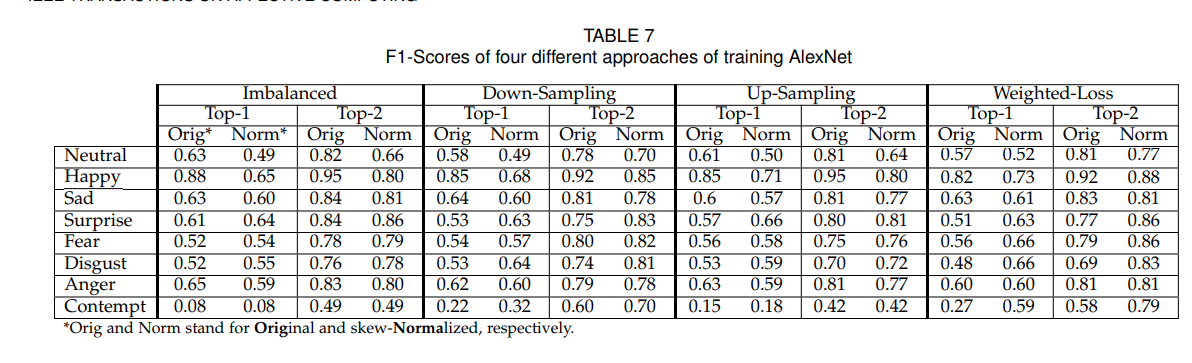
\includegraphics[width=15cm]{fscore}
	
	\caption{Top 2 F1-score}
	\label{Fig:t7}
	%插入图片的标题,一般放在图片的下方,放在表格的上方
\end{figure}

直接对数据集进行训练,样本较少的表交叉较差,采取了加权损失函数之后,F1 score有所提高。

\subsubsection{加权损失函数下Confusion Matrix}

由图\ref{Fig:t7}可得出,加权损失函下,总体F-score的表现较好,测试集的Confusion Matrix的结果如下:

\begin{figure}[htbp]
	
	\centering %使插入的图片居中显示
	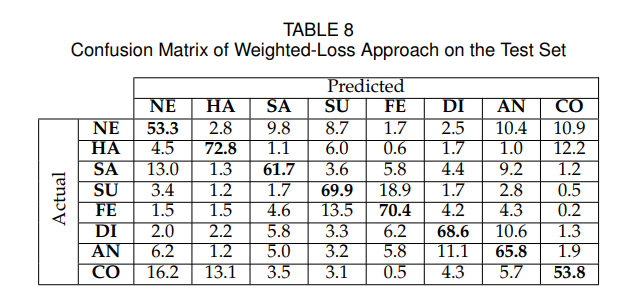
\includegraphics[width=13cm]{table8}
	
	\caption{测试集 Confusion Matrix, 在加权损失函数下}
	\label{Fig:t8}
	%插入图片的标题,一般放在图片的下方,放在表格的上方
\end{figure}

\subsubsection{几种不同的评判标准}

以下几种标准均用于二分类模型,此处是将正确分类的结果总结为第1类,错误的结果第二类,在准确率的基础上对Baseline的结果进行评测。

\newpage
\begin{itemize}
\item F1 Score
\item Cohen's Kappa 评判分类准确性,区间[0,1]
\item Krippendorfs Alpha 评判分类准确性,区间[0,1]
\item Area under the ROC curve (AUC)  区间[0,1]低于0.6说明模型效果很差
\item Area under the Precision-Recall curve (AUC-PR),区间[0,1]
\end{itemize}


\begin{figure}[htbp]
	
	\centering %使插入的图片居中显示
	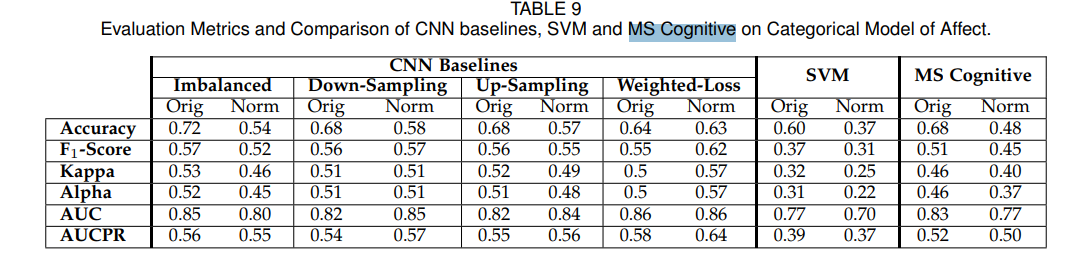
\includegraphics[width=15cm]{table9}
	
	\caption{Baseline的不同评判标准}
	\label{Fig:t9}
	%插入图片的标题,一般放在图片的下方,放在表格的上方
\end{figure}

\subsection{Dimensional Model Baseline}
针对表情的维度模型中,另一种是基于Arousal(情绪的强烈程度)和Valence(情绪的正负倾向)。

AlexNet作为回归模型,最后的全连接被替代为仅含有一个神经元的线性回归层。

输出数值的范围在[-1,1]之间。所采取的损失函数为欧式距离。损失函数定义如下:

\begin{equation}
E = \frac{1}{2N}\sum_{N}^{n=1} {\begin{Vmatrix}
\hat{y_n} - y_n\\ 
\end{Vmatrix}}^2_2
\end{equation}

在回归模型中,图片被剪切为256$\times$256。回归模型的相关参数:

\begin{itemize}
	\item Epoch: 16
	\item Batch Size: 256
	\item Learning Rate: 0.001 
	\item Momentum: 0.9
\end{itemize}

\subsubsection{评判标准}

\begin{itemize}
\item RMSE Root Mean Square Error
\item CORR Pearson's Correlation Coefficient
\item Concordance Correlation Coefficient (CCC)
\end{itemize}

具体结果见于图\ref{Fig:t10}中。其中同时给了基于支持向量机的回归模型。AlexNet的结果优于SVR。

\begin{figure}[htbp]
	
	\centering %使插入的图片居中显示
	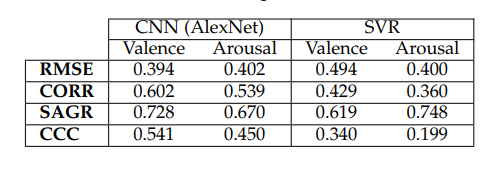
\includegraphics[width=15cm]{table10}
	
	\caption{Baseline的不同评判标准}
	\label{Fig:t10}
	%插入图片的标题,一般放在图片的下方,放在表格的上方
\end{figure}


\section{ResNet18 Training Result (Using Keras)}

基于resnet模型训练结果如下(增加了Batch Normalization层,在每次卷积之后):

一些参数:

\begin{itemize}
\item Epoch : 30
\item batch size: 16
\item Learning Rate: 0.01 
\item L2 Regularizer: 0.0001 (1e-4)
\item Optimizer: Adam
\end{itemize}

模型在训练集和验证集的结果如下:

	\begin{figure}[htbp]
		
		\centering %使插入的图片居中显示
		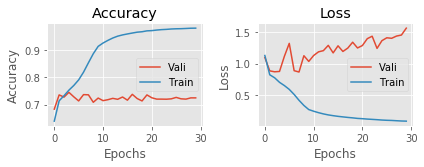
\includegraphics[width=12cm]{resnet34}
		
		\caption{ReseNet34 结果,增加了BN层}
		\label{Fig:result}
		%插入图片的标题,一般放在图片的下方,放在表格的上方
	\end{figure}

测试集的结果:

Loss: 1.67 Accuracy: 71.2\%
	
\section{其他结果}
\subsection{Paper Result}
目前只查到一篇report,作者对8分类和3分类,RGB和灰度图像进行了训练。

三分类是将表情几种分类为Positive,nagative和neutral.
http://lup.lub.lu.se/luur/download?func=downloadFile\&recordOId=8943330\&fileOId=8943332

\subsubsection{8分类,验证集}

	\begin{figure}[htbp]
	
	\centering %使插入的图片居中显示
	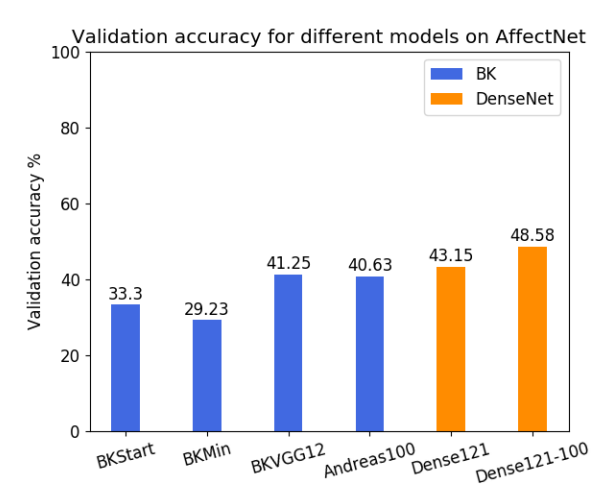
\includegraphics[width=8cm]{result}
	
	\caption{ReseNet34 结果,增加了BN层}
	\label{Fig:result2}
	%插入图片的标题,一般放在图片的下方,放在表格的上方
\end{figure}

\subsubsection{8分类和3分类,验证集}

模型为BKVGG12,结果为8分类和3分类,灰度和RGB。

\newpage

\begin{figure}[htbp]
	
	\centering %使插入的图片居中显示
	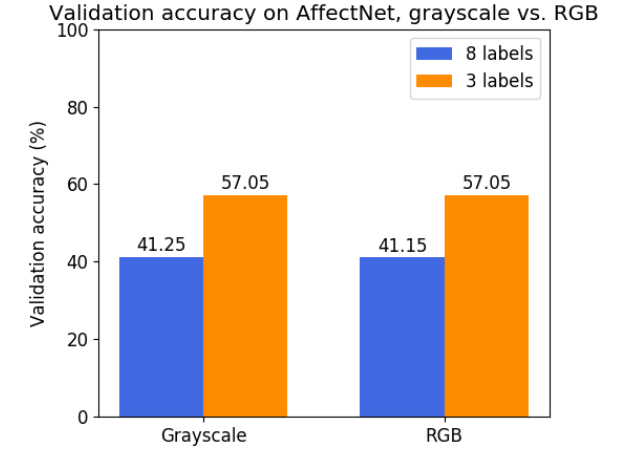
\includegraphics[width=8cm]{result2}
	
	\caption{ReseNet34 结果,增加了BN层}
	\label{Fig:result3}
	%插入图片的标题,一般放在图片的下方,放在表格的上方
\end{figure}

\subsubsection{Confusion Matrix}

Confusion Matrix:

\begin{figure}[htbp]
	
	\centering %使插入的图片居中显示
	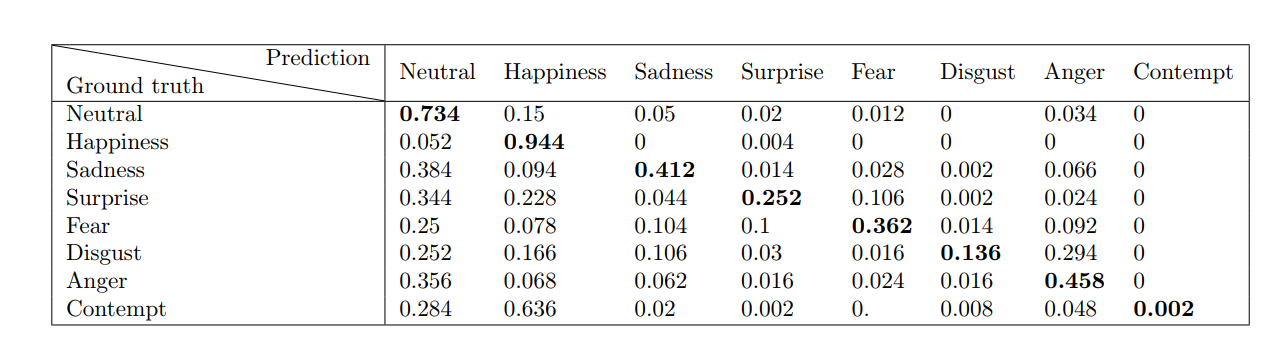
\includegraphics[width=15cm]{confusion}
	
	\caption{3/8分类,灰度和RGB}
	\label{Fig:cm}
	%插入图片的标题,一般放在图片的下方,放在表格的上方
\end{figure}


\subsection{中文网络}
查到一篇博客,使用AlexNet,训练集的准确度为70\%,验证集38\%.

resource:
https://blog.csdn.net/ZWX2445205419/article/details/79086288

\section{总结}

从不同的训练结果来看,Happiness和Neutral模型识别的能力比较高。

Disgust, Contempt和Disgust三种表情分类识别能力较弱。
\end{CJK}


%\tableofcontents

%\listoffigures
%\listoftables
%\lstlistoflistings        


%\newpage




\bibliographystyle{IEEEtran}  
%\bibliography{MyRefs} 
%\addcontentsline{toc}{section}{References}





%-------------------------------------------------------------------------------------------------------





\end{document}
